%%%%%%%%%%%%  Generated using docx2latex.com  %%%%%%%%%%%%%%

%%%%%%%%%%%%  v2.0.0-beta  %%%%%%%%%%%%%%

\documentclass[12pt]{article}
\usepackage{amsmath}
\usepackage{latexsym}
\usepackage{amsfonts}
\usepackage[normalem]{ulem}
\usepackage{array}
\usepackage{amssymb}
\usepackage{graphicx}
\usepackage[backend=biber,
style=numeric,
sorting=none,
isbn=false,
doi=false,
url=false,
]{biblatex}\addbibresource{bibliography.bib}

\usepackage{subfig}
\usepackage{wrapfig}
\usepackage{wasysym}
\usepackage{enumitem}
\usepackage{adjustbox}
\usepackage{ragged2e}
\usepackage[svgnames,table]{xcolor}
\usepackage{tikz}
\usepackage{longtable}
\usepackage{changepage}
\usepackage{setspace}
\usepackage{hhline}
\usepackage{multicol}
\usepackage{tabto}
\usepackage{float}
\usepackage{multirow}
\usepackage{makecell}
\usepackage{fancyhdr}
\usepackage[toc,page]{appendix}
\usepackage[hidelinks]{hyperref}
\usetikzlibrary{shapes.symbols,shapes.geometric,shadows,arrows.meta}
\tikzset{>={Latex[width=1.5mm,length=2mm]}}
\usepackage{flowchart}\usepackage[paperheight=11.69in,paperwidth=8.27in,left=0.98in,right=0.98in,top=0.98in,bottom=0.98in,headheight=1in]{geometry}
\usepackage[utf8]{inputenc}
\usepackage[T1]{fontenc}
\TabPositions{0.49in,0.98in,1.47in,1.96in,2.45in,2.94in,3.43in,3.92in,4.41in,4.9in,5.39in,5.88in,}

\urlstyle{same}
%%%%%%%%%%%%%%%%%%%%% CoverPage %%%%%%%%%%%

\begin{titlepage}

\newcommand{\HRule}{\rule{\linewidth}{0.5mm}} % Defines a new command for the horizontal lines, change thickness here

\center % Center everything on the page
 
%----------------------------------------------------------------------------------------
%	HEADING SECTIONS
%----------------------------------------------------------------------------------------

\textsc{\LARGE Université Paris 13}\\[1.5cm] % Name of your university/college
\textsc{\Large Institut Galilée}\\[0.5cm] % Major heading such as course name
\textsc{\large Master 2 : Exploration informatique des données et décisionnel}\\[0.5cm] % Minor heading such as course title

%----------------------------------------------------------------------------------------
%	TITLE SECTION
%----------------------------------------------------------------------------------------

\HRule \\[0.4cm]
{ \huge \bfseries Scala tutoriels}\\[0.4cm]
{ \huge \bfseries scalaTest and uTest}\\[0.2cm]
% Title of your document
\HRule \\[1.5cm]
 
%----------------------------------------------------------------------------------------
%	AUTHOR SECTION
%----------------------------------------------------------------------------------------

\begin{minipage}{0.4\textwidth}
\begin{flushleft} \large
\emph{Rédigé par:}\\
LEZARK Halima (uTest)
SEDDIKI Hanae (ScalaTest)% Your name
\end{flushleft}
\end{minipage}
~
\begin{minipage}{0.3\textwidth}
\begin{flushright} \large
\emph{Supervisé par:} \\
Mr. BOUDES Pierre % Supervisor's Name
\end{flushright}
\end{minipage}\\[2cm]

% If you don't want a supervisor, uncomment the two lines below and remove the section above
%\Large \emph{Author:}\\
%John \textsc{Smith}\\[3cm] % Your name

%----------------------------------------------------------------------------------------
%	DATE SECTION
%----------------------------------------------------------------------------------------

{\large \today}\\[0.3cm] % Date, change the \today to a set date if you want to be precise

%----------------------------------------------------------------------------------------
%	LOGO SECTION
%----------------------------------------------------------------------------------------


\includegraphics{./media/image1.png}\\[1cm] % Include a department/university logo - this will require the graphicx package
 
%----------------------------------------------------------------------------------------

\vfill % Fill the rest of the page with whitespace

\end{titlepage}

%%%%%%%%%%%%%%%%%%%%% CoverPage %%%%%%%%%%%%%

 %%%%%%%%%%%%  Set Depths for Sections  %%%%%%%%%%%%%%
\tableofcontents



 %%%%%%%%%%%%  Set Depths for Nested Lists created by \begin{enumerate}  %%%%%%%%%%%%%%


\setlistdepth{9}
\renewlist{enumerate}{enumerate}{9}
		\setlist[enumerate,1]{label=\arabic*)}
		\setlist[enumerate,2]{label=\alph*)}
		\setlist[enumerate,3]{label=(\roman*)}
		\setlist[enumerate,4]{label=(\arabic*)}
		\setlist[enumerate,5]{label=(\Alph*)}
		\setlist[enumerate,6]{label=(\Roman*)}
		\setlist[enumerate,7]{label=\arabic*}
		\setlist[enumerate,8]{label=\alph*}
		\setlist[enumerate,9]{label=\roman*}

\renewlist{itemize}{itemize}{9}
		\setlist[itemize]{label=$\cdot$}
		\setlist[itemize,1]{label=\textbullet}
		\setlist[itemize,2]{label=$\circ$}
		\setlist[itemize,3]{label=$\ast$}
		\setlist[itemize,4]{label=$\dagger$}
		\setlist[itemize,5]{label=$\triangleright$}
		\setlist[itemize,6]{label=$\bigstar$}
		\setlist[itemize,7]{label=$\blacklozenge$}
		\setlist[itemize,8]{label=$\prime$}



 %%%%%%%%%%%%  Header here  %%%%%%%%%%%%%%


\pagestyle{fancy}
\fancyhf{}
\cfoot{ 
\vspace{\baselineskip}
}
\renewcommand{\headrulewidth}{0pt}
\setlength{\topsep}{0pt}\setlength{\parskip}{8.04pt}
\setlength{\parindent}{0pt}

 %%%%%%%%%%%%  This sets linespacing (verticle gap between Lines) Default=1 %%%%%%%%%%%%%%


\renewcommand{\arraystretch}{1.3}


%%%%%%%%%%%%%%%%%%%% Document code starts here %%%%%%%%%%%%%%%%%%%%



\begin{document}




 %%%%%%%%%%%%  Starting New Page here %%%%%%%%%%%%%%

\newpage

\vspace{\baselineskip}\section{Préparation de l’environnement de travail}

\vspace{\baselineskip}
\begin{justify}
Avant de commencer le développement du projet, nous avons besoin de préparer un environnement de travail.
\end{justify}\par

\begin{justify}
Dans ce tutoriel, nous allons travailler sur linux et avec l’IDE IntelliJ IDEA.
\end{justify}\par

\begin{justify}
Pour se faire, nous commençons par l’installation du JDK, un environnement d'exécution dans lequel les programmes Scala sont exécutés.
\end{justify}\par

\begin{justify}
On utilise la commande : \colorbox{Cyan}{sudo apt-get install open jdk-8-jdk} pour installer jdk.
\end{justify}\par

\begin{justify}
Ensuite, on installe \href{https://www.jetbrains.com/idea/download/}{IntelliJ Ultimate}. Lorsque vous démarrez Intellij, un écran de bienvenue s’affiche. La première étape avant de créer ou d’ouvrir un projet Scala consiste à installer le plugin Scala. Pour cela, allez-vous-en bas à droite de l'écran de bienvenue et choisissez \textcolor[HTML]{373A3C}{Configure $ \rightarrow $  Plugins $ \rightarrow $  Browse JetBrains Plugins. }Si cet écran de bienvenue ne s'affiche pas, allez à\textcolor[HTML]{373A3C}{ Préférences (Settings) $ \rightarrow $  Plugins.}
\end{justify}\par

\begin{justify}
Par conséquent, \textbf{redémarrez IntelliJ} avant de suivre les autres étapes.
\end{justify}\par

\subsection{Configuration du JDK}


Sur l’écran de bienvenue, sur \textcolor[HTML]{373A3C}{Configure $ \rightarrow $  Project defaults $ \rightarrow $  Project structure et ajouter JDK qui sera automatiquement ajouté, sinon, trouvez le chemin où il est stocké et sélectionnez-le dans le sélecteur de fichiers.}\par

\subsection{SBT}

\textcolor[HTML]{222222}{SBT est un outil de construction open source pour les projets Scala et Java, similaire à Maven et Ant de Java. Ses principales caractéristiques sont : Prise en charge native de la compilation de code Scala et de l'intégration à de nombreux frameworks de test Scala Compilation, test et déploiement continus.}\par

\subsection{Création du projet}

La création du projet consiste à utiliser l’Assistant de projet. Pour l'utiliser, cliquez sur Créer un nouveau projet sur l'écran de bienvenue, puis sélectionnez \textbf{Scala} et enfin \textbf{Projet SBT}.\par



%%%%%%%%%%%%%%%%%%%% Figure/Image No: 1 starts here %%%%%%%%%%%%%%%%%%%%

\begin{figure}[H]
	\begin{Center}
		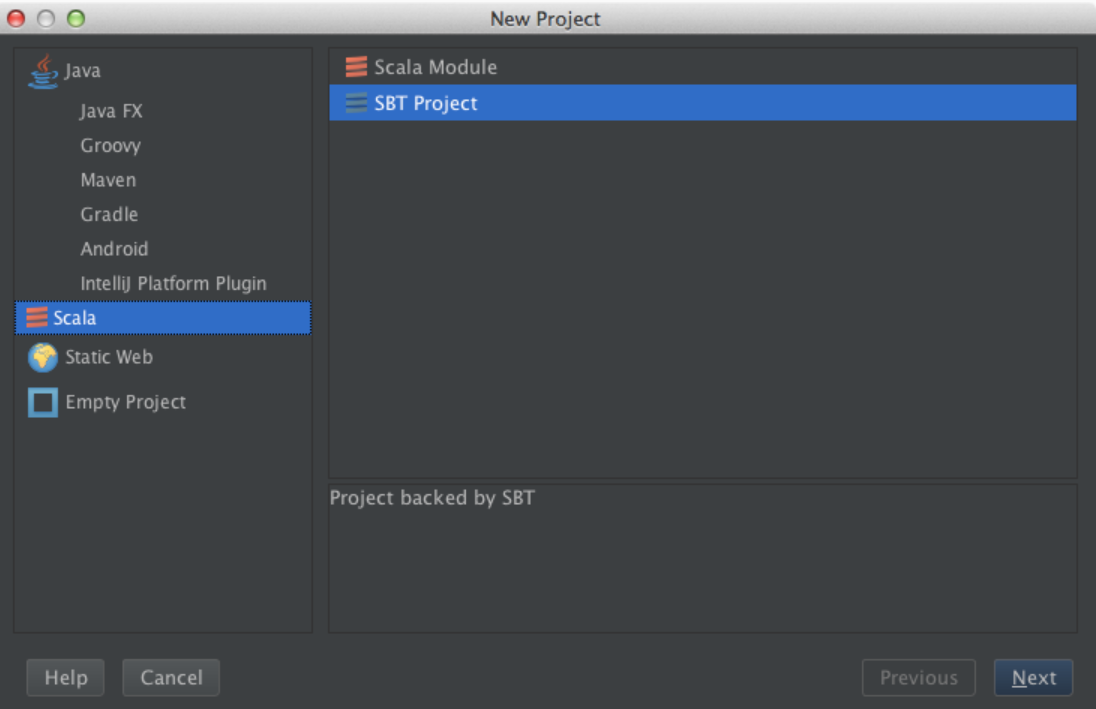
\includegraphics[width=3.47in,height=2.24in]{./media/image2.png}
	\end{Center}
\end{figure}


%%%%%%%%%%%%%%%%%%%% Figure/Image No: 1 Ends here %%%%%%%%%%%%%%%%%%%%

\par

Cliquez sur Suivant pour spécifier le nom et l'emplacement du projet. Une fois ces informations saisies, IntelliJ IDEA créera un projet vide contenant un fichier build.sbt.\par

\section{UTest : un Framework pour les tests de scala}

\subsection{Présentation des uTest :}

\begin{justify}
uTest est un Framework de test pour le langage de programmation Scala. uTest est simple et convivial, il permet de se concentrer sur l'essentiel: les tests et le code. 
\end{justify}\par

\begin{justify}
Dans cette partie, on va explorer ce qui rend uTest intéressant et pourquoi on doit envisager de l'utiliser pour créer la suite de tests dans les projets Scala.
\end{justify}\par

\begin{justify}
uTest n'est pas "essentiel" dans le sens où vous devez l'utiliser: d'autres Framework de test comme ScalaTest ou Specs2 sont toujours une option. Au lieu de cela, uTest est essentiel car il ne contient que les fonctionnalités qui sont absolument nécessaires pour tester votre code.
\end{justify}\par

uTest prend en charge les tâches suivantes:\par

\begin{itemize}
	\item Écrire des bouts de code à exécuter ("tests"), les étiqueter et les organiser soigneusement\par

	\item Partage de l'initialisation et d'autres codes entre vos différents tests\par

	\item Affirmer des choses pour s'assurer qu'elles sont vraies\par

	\item Sélectionner les tests que vous voulez exécuter et voir s'ils explosent
\end{itemize}\par


\vspace{\baselineskip}
\subsection{C’est quoi un TestSuit ?}

\begin{justify}
Un testSuit est un conteneur qui contient un ensemble de tests qui aide les testeurs à exécuter et à signaler l'état d'exécution des tests. Cela peut prendre n'importe lequel des trois états, à savoir Actif, In Progress et complété.
\end{justify}\par

\begin{justify}
Un scénario de test peut être ajouté à plusieurs suites de tests et plans de tests. Après avoir créé un plan de test, des suites de tests sont créées et peuvent comporter un nombre illimité de tests.
\end{justify}\par

\subsection{Pour Commencer }

\begin{justify}
La plupart des gens qui utilisent uTest exécuteront des tests via SBT. 
\end{justify}\par

\begin{justify}
On doit faire la modification nécessaire au fichier build.sbt et on peut immédiatement commencer à définir et exécuter des tests par programmation.
\end{justify}\par

\begin{justify}
Dès la création du projet scala, le fichier build.sbt se génère automatiquement, ainsi qu’un dossier src contenant deux dossiers : main et test.
\end{justify}\par

\begin{justify}
Dans le dossier main, on crée des classes scala où on met le code et dans le dossier test on met les objets scala contenant les tests.
\end{justify}\par



%%%%%%%%%%%%%%%%%%%% Figure/Image No: 2 starts here %%%%%%%%%%%%%%%%%%%%

\begin{figure}[H]
	\begin{Center}
		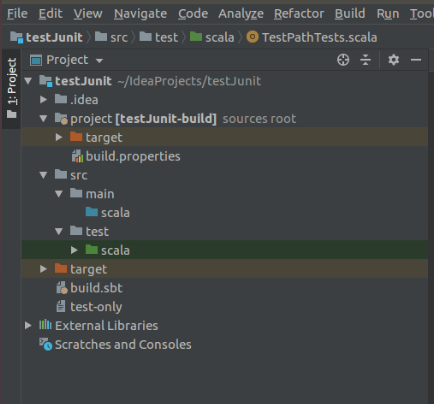
\includegraphics[width=3.12in,height=2.9in]{./media/image3.png}
	\end{Center}
\end{figure}


%%%%%%%%%%%%%%%%%%%% Figure/Image No: 2 Ends here %%%%%%%%%%%%%%%%%%%%

\par

\subsubsection{Définir et exécuter un TestSuite}

Dans le dossier src / test / scala / , on met :\par



%%%%%%%%%%%%%%%%%%%% Figure/Image No: 3 starts here %%%%%%%%%%%%%%%%%%%%

\begin{figure}[H]
	\begin{Center}
		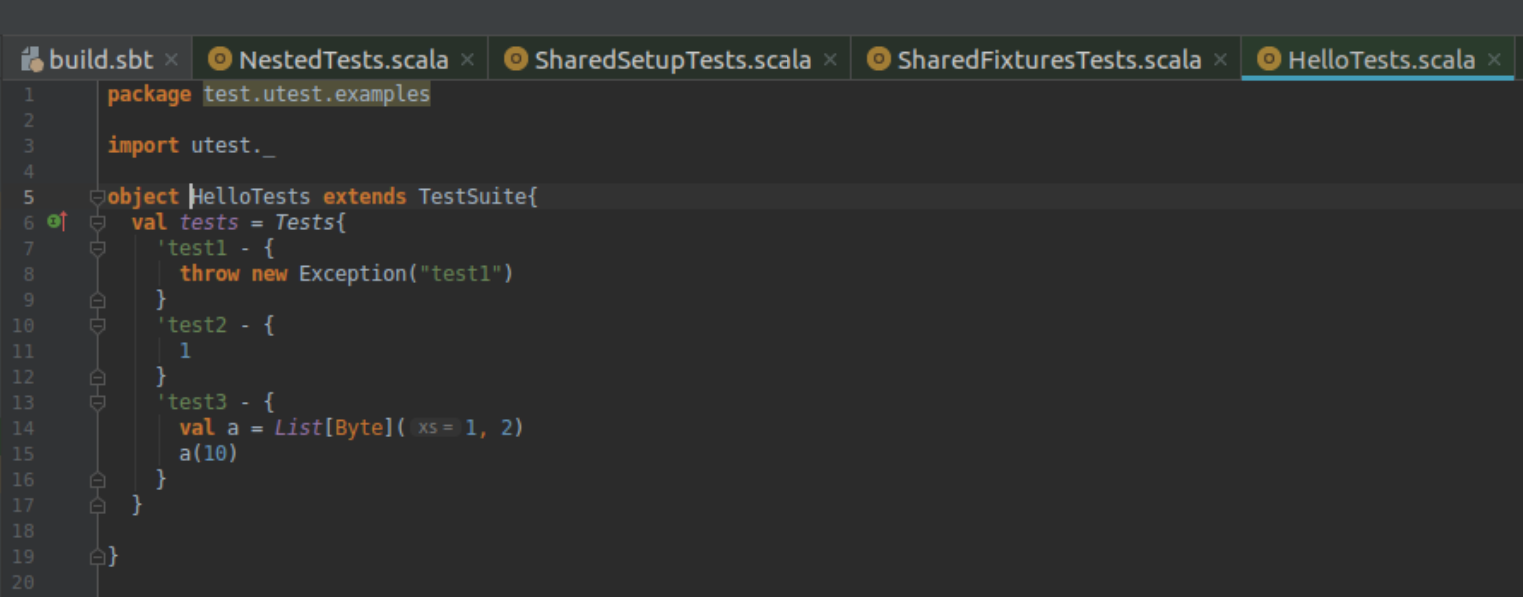
\includegraphics[width=5.06in,height=1.98in]{./media/image4.png}
	\end{Center}
\end{figure}


%%%%%%%%%%%%%%%%%%%% Figure/Image No: 3 Ends here %%%%%%%%%%%%%%%%%%%%

\par

Vous pouvez ensuite exécuter ceci :\par

\colorbox{Cyan}{sbt testJunit/test}\par



%%%%%%%%%%%%%%%%%%%% Figure/Image No: 4 starts here %%%%%%%%%%%%%%%%%%%%

\begin{figure}[H]
	\begin{Center}
		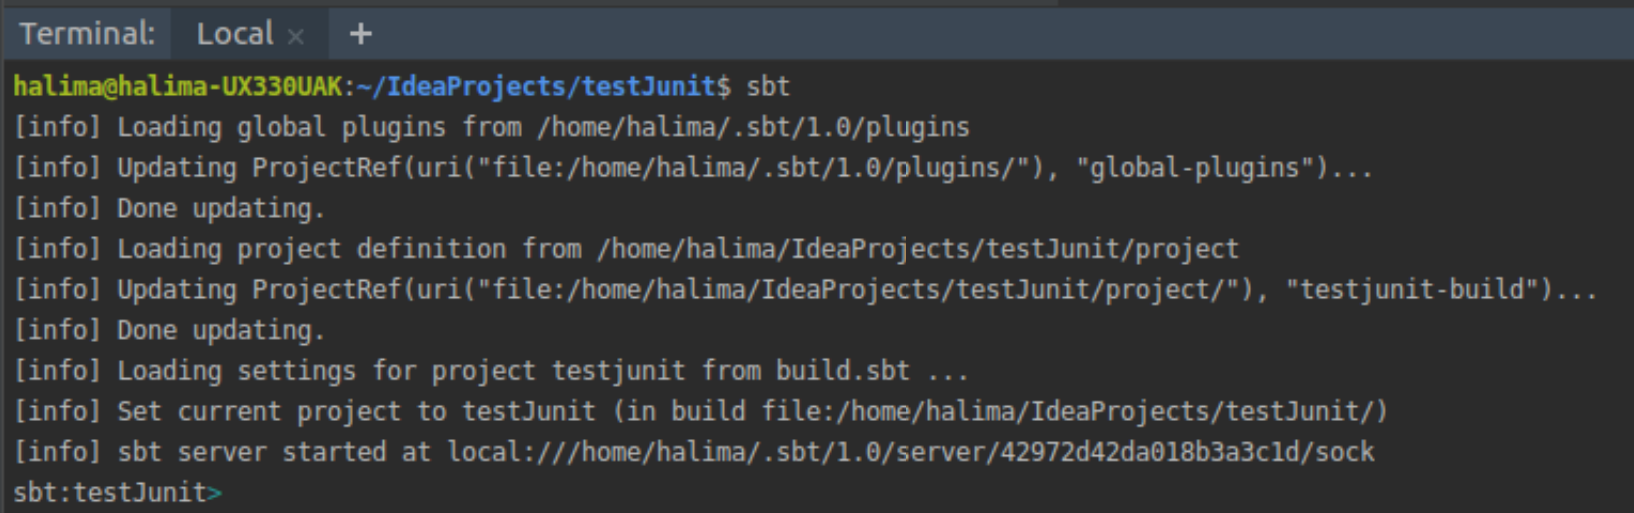
\includegraphics[width=5.26in,height=1.65in]{./media/image5.png}
	\end{Center}
\end{figure}


%%%%%%%%%%%%%%%%%%%% Figure/Image No: 4 Ends here %%%%%%%%%%%%%%%%%%%%

\par

On lance le test sur l’objet HelloTests, on obtient :\par



%%%%%%%%%%%%%%%%%%%% Figure/Image No: 5 starts here %%%%%%%%%%%%%%%%%%%%

\begin{figure}[H]
	\begin{Center}
		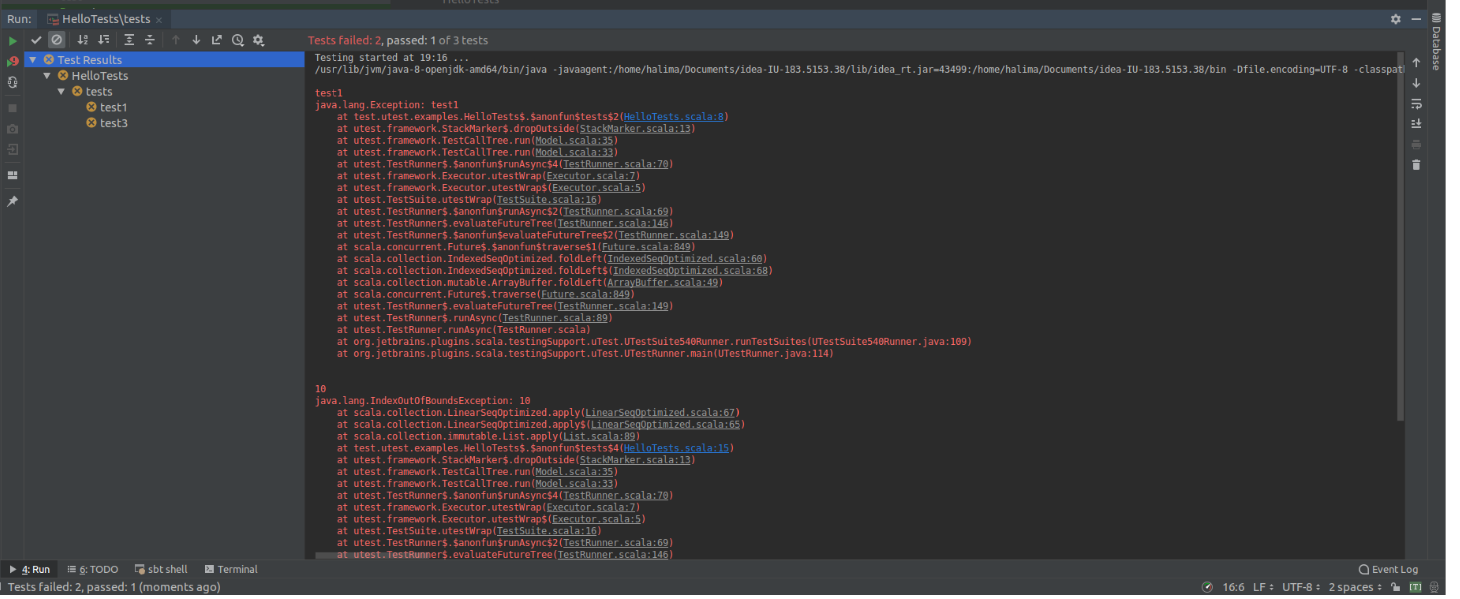
\includegraphics[width=6.12in,height=2.68in]{./media/image6.png}
	\end{Center}
\end{figure}


%%%%%%%%%%%%%%%%%%%% Figure/Image No: 5 Ends here %%%%%%%%%%%%%%%%%%%%

\par

\begin{itemize}
	\item 3 tests exécutés, 1 test réussi et 2 deux tests ont échoués. \par


\end{itemize}\subsubsection{Tests d'imbrication (Nesting tests) }

\begin{justify}
Notez que les tests de la suite peuvent être imbriqués les uns dans les autres, mais uniquement directement. Par exemple. Vous ne pouvez pas définir de tests dans les instructions if ou for-loops.
\end{justify}\par

\begin{justify}
uTest s'appuie sur la structure de test pour être connue statiquement au moment de la compilation.
\end{justify}\par



%%%%%%%%%%%%%%%%%%%% Figure/Image No: 6 starts here %%%%%%%%%%%%%%%%%%%%

\begin{figure}[H]
	\begin{Center}
		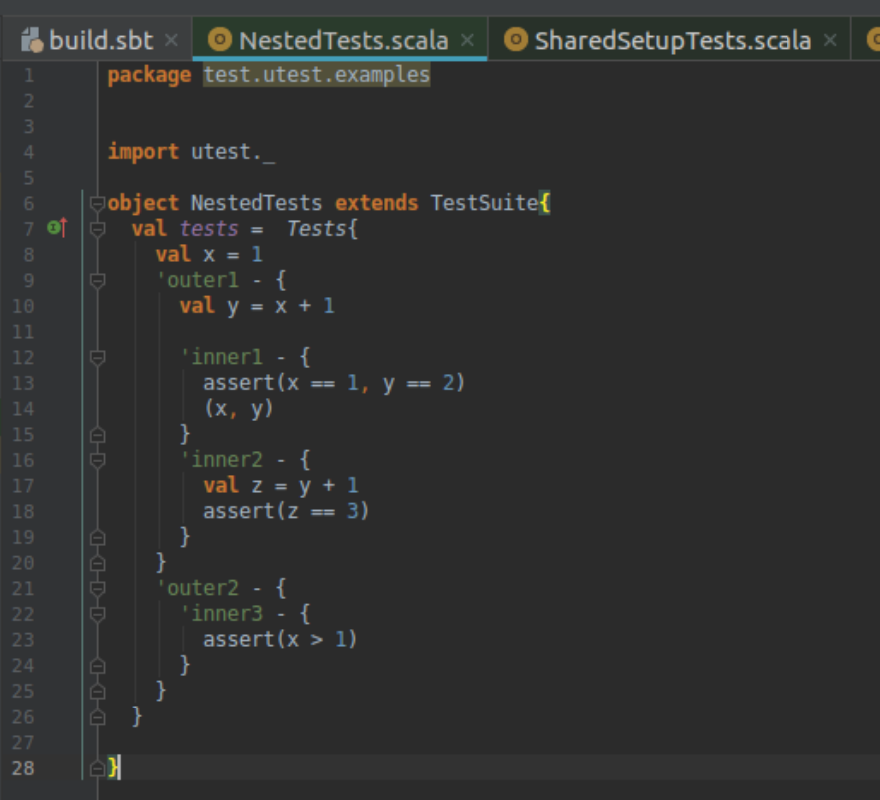
\includegraphics[width=2.78in,height=2.53in]{./media/image7.png}
	\end{Center}
\end{figure}


%%%%%%%%%%%%%%%%%%%% Figure/Image No: 6 Ends here %%%%%%%%%%%%%%%%%%%%

\par

Après exécution, on obtient :\par



%%%%%%%%%%%%%%%%%%%% Figure/Image No: 7 starts here %%%%%%%%%%%%%%%%%%%%

\begin{figure}[H]
	\begin{Center}
		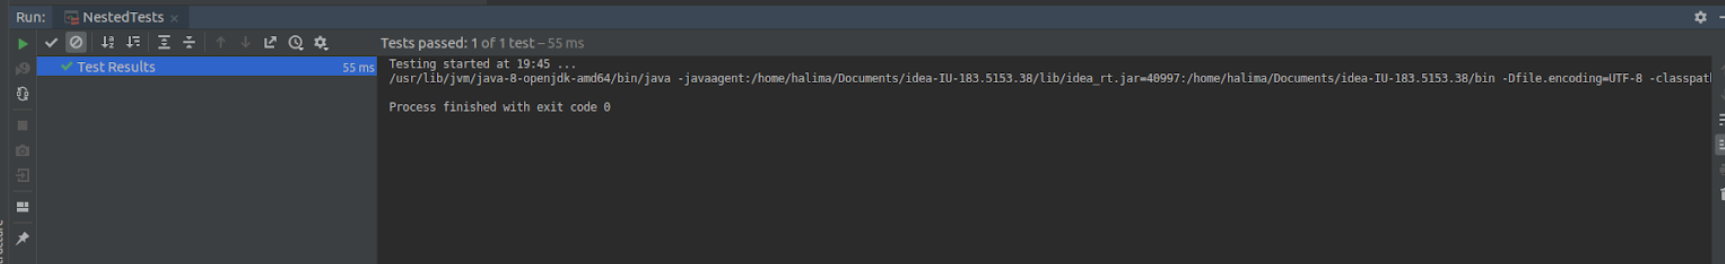
\includegraphics[width=6.3in,height=0.96in]{./media/image8.png}
	\end{Center}
\end{figure}


%%%%%%%%%%%%%%%%%%%% Figure/Image No: 7 Ends here %%%%%%%%%%%%%%%%%%%%

\par

\begin{itemize}
	\item 4\ tests exécutés => 4 Réussis  \par

\begin{justify}
Comme vous pouvez le constater, les trois éléments différents sont imbriqués les uns dans les autres.
\end{justify}\par


\end{itemize}\subsubsection{Tests de Partage de la configuration (Sharing Setup tests) }

\begin{justify}
Vous pouvez utiliser les tests imbriqués pour regrouper les tests associés et les faire partager.
\end{justify}\par



%%%%%%%%%%%%%%%%%%%% Figure/Image No: 8 starts here %%%%%%%%%%%%%%%%%%%%

\begin{figure}[H]
	\begin{Center}
		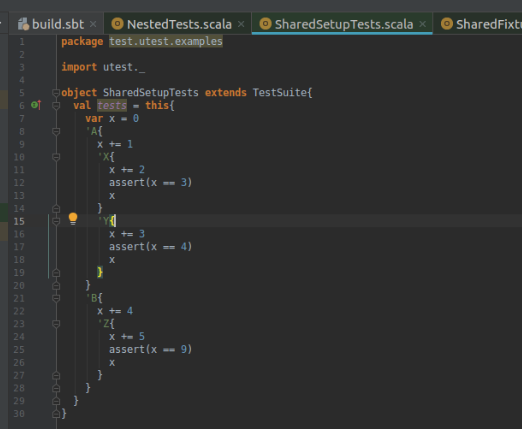
\includegraphics[width=3.2in,height=2.63in]{./media/image9.png}
	\end{Center}
\end{figure}


%%%%%%%%%%%%%%%%%%%% Figure/Image No: 8 Ends here %%%%%%%%%%%%%%%%%%%%

\par

\begin{itemize}
	\item Cela donnera :\par



%%%%%%%%%%%%%%%%%%%% Figure/Image No: 9 starts here %%%%%%%%%%%%%%%%%%%%

\begin{figure}[H]
	\begin{Center}
		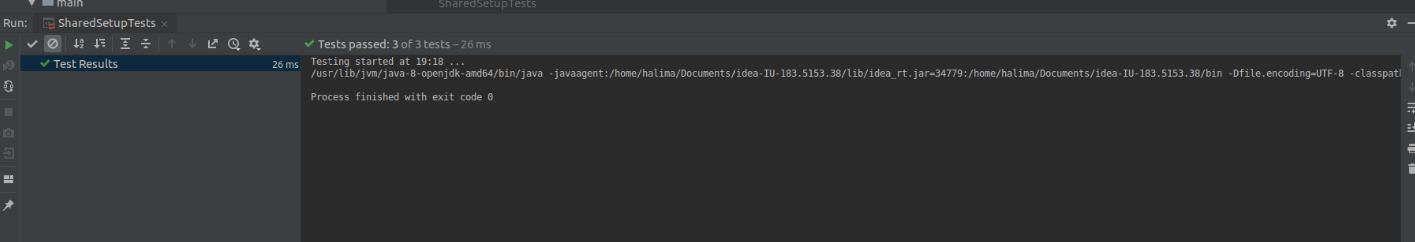
\includegraphics[width=6.78in,height=1.24in]{./media/image10.png}
	\end{Center}
\end{figure}


%%%%%%%%%%%%%%%%%%%% Figure/Image No: 9 Ends here %%%%%%%%%%%%%%%%%%%%

\par

\begin{justify}
Ici, nous partageons l’initialisation de la variable x entre tous les différents sous-tests dans le même dossier.
\end{justify}\par

\begin{justify}
Bien qu’ils soient partagés lexicalement, ces helpers sont recréés pour chaque test qui est exécuté, donc si elles contiennent un état mutable (par exemple, des collections mutables ou vars) vous n'avez pas à vous soucier des mutations de plusieurs tests qui interfèrent entre eux.
\end{justify}\par

\begin{justify}
Cela permet de partager de manière concise un code de configuration commun entre tests liés dans le même groupe, tout en évitant les interférences entre les tests en raison de la mutation des appareils partagés
\end{justify}\par

\begin{justify}
Si vous voulez que les rencontres soient vraiment partagé entre différents tests, définissez-le en dehors du bloc this $ \{ $ $ \} $ :
\end{justify}\par



%%%%%%%%%%%%%%%%%%%% Figure/Image No: 10 starts here %%%%%%%%%%%%%%%%%%%%

\begin{figure}[H]
	\begin{Center}
		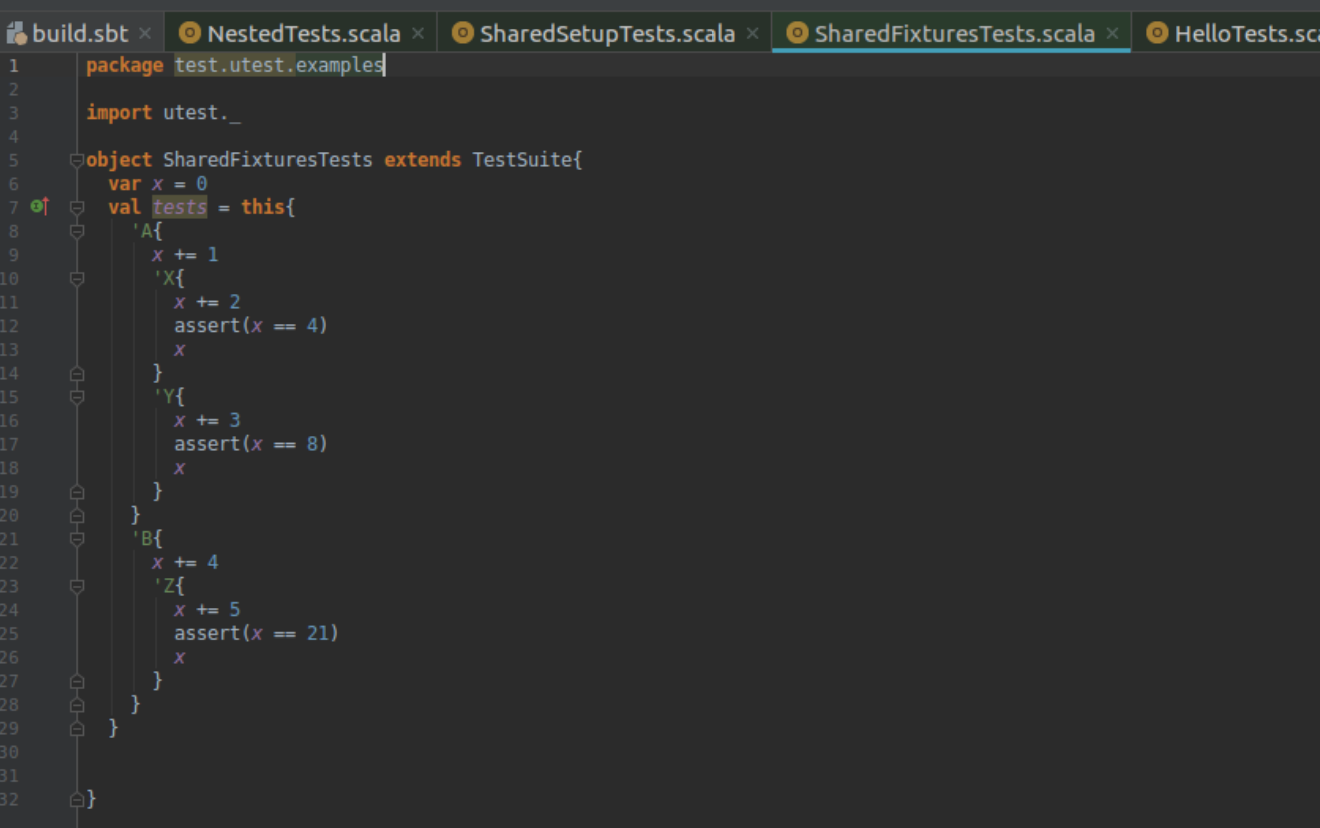
\includegraphics[width=4.57in,height=2.87in]{./media/image11.png}
	\end{Center}
\end{figure}


%%%%%%%%%%%%%%%%%%%% Figure/Image No: 10 Ends here %%%%%%%%%%%%%%%%%%%%

\par

	\item Après exécution :\par



%%%%%%%%%%%%%%%%%%%% Figure/Image No: 11 starts here %%%%%%%%%%%%%%%%%%%%

\begin{figure}[H]
	\begin{Center}
		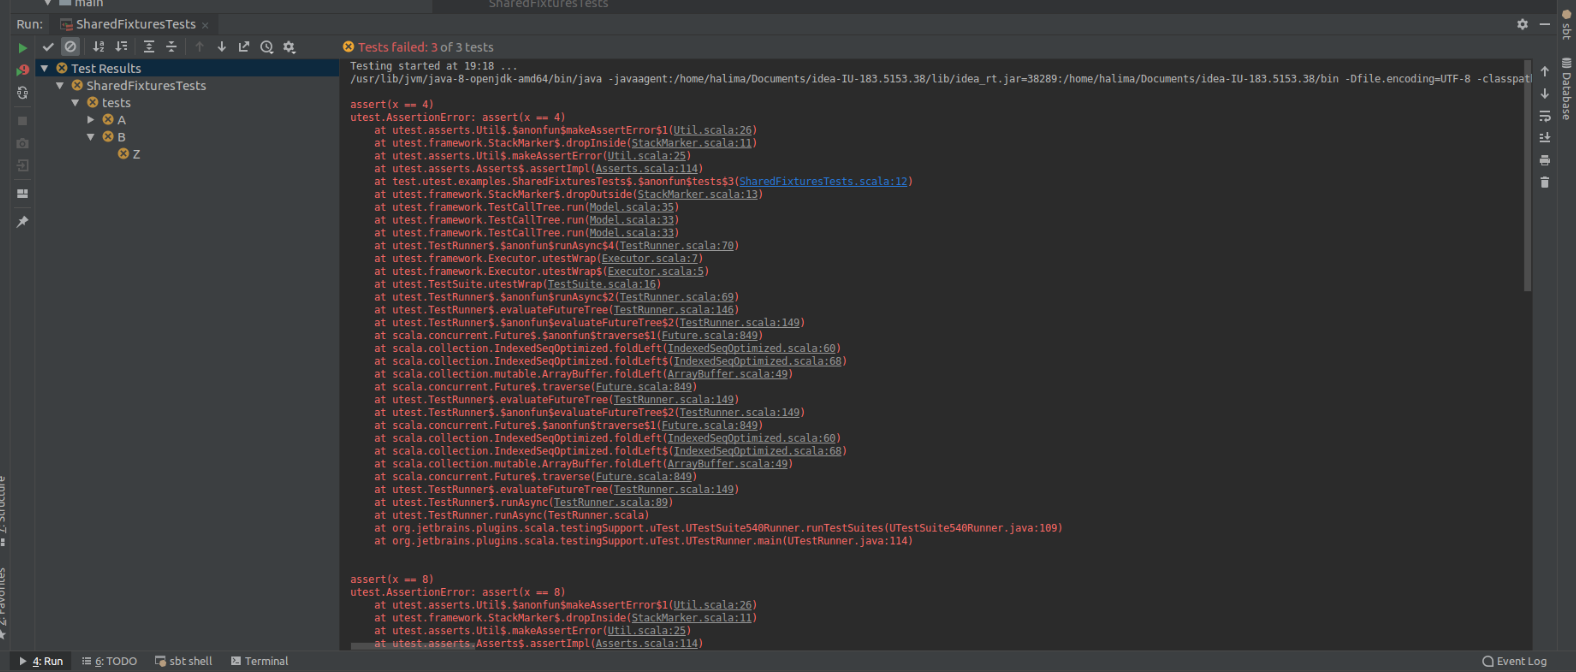
\includegraphics[width=5.49in,height=2.34in]{./media/image12.png}
	\end{Center}
\end{figure}


%%%%%%%%%%%%%%%%%%%% Figure/Image No: 11 Ends here %%%%%%%%%%%%%%%%%%%%

\par

\begin{justify}
Et vous verrez que les modifications apportées à x sont partagées entre l’invocation de tous les tests : A l'incrémente de 1, X de 1 puis 2, à 4, Y par 1 et 3 à 8, et ainsi de suite.
\end{justify}\par

\begin{justify}
Cela vous permet d'éviter de refaire le travail plusieurs fois.
\end{justify}\par


\end{itemize}\subsubsection{Les utilitaires de test}

\begin{justify}
uTest fournit une gamme d’utilitaires de test qui ne sont pas strictement nécessaires, mais visez à rendre l’écriture des tests beaucoup plus pratique.
\end{justify}\par

\begin{justify}
\textbf{TestPath}
\end{justify}\par



%%%%%%%%%%%%%%%%%%%% Figure/Image No: 12 starts here %%%%%%%%%%%%%%%%%%%%

\begin{figure}[H]
	\begin{Center}
		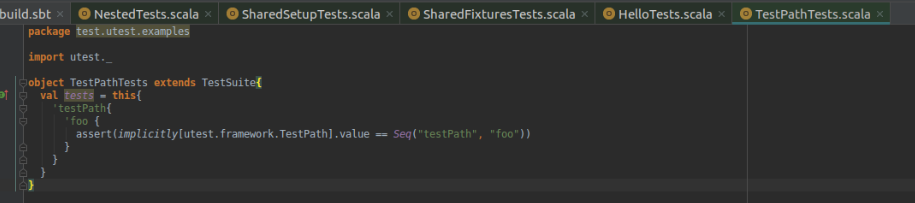
\includegraphics[width=6.3in,height=1.4in]{./media/image13.png}
	\end{Center}
\end{figure}


%%%%%%%%%%%%%%%%%%%% Figure/Image No: 12 Ends here %%%%%%%%%%%%%%%%%%%%

\par

\begin{itemize}
	\item Cela donne comme résultat :
\end{itemize}\par



%%%%%%%%%%%%%%%%%%%% Figure/Image No: 13 starts here %%%%%%%%%%%%%%%%%%%%

\begin{figure}[H]
	\begin{Center}
		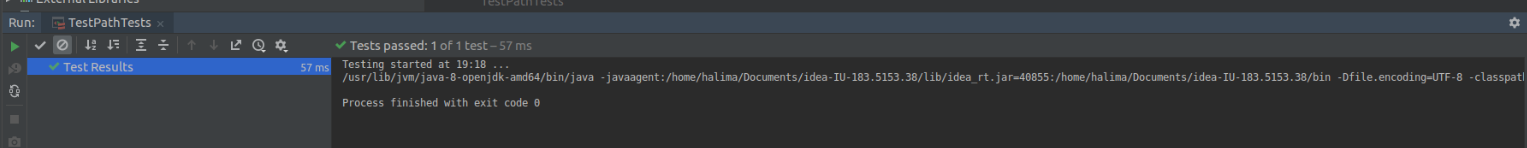
\includegraphics[width=6.3in,height=0.69in]{./media/image14.png}
	\end{Center}
\end{figure}


%%%%%%%%%%%%%%%%%%%% Figure/Image No: 13 Ends here %%%%%%%%%%%%%%%%%%%%

\par


\vspace{\baselineskip}
uTest expose le corps du test au chemin du test en cours via le utest.framework.TestPath implicite.\par

\section{ScalaTest}

\subsection{Le premier pas avec ScalaTest}

ScalaTest est l'outil de test le plus flexible et le plus populaire de l'écosystème Scala. Avec ScalaTest, vous pouvez tester le code Scala, Scala.js (JavaScript) et Java.\par

Pour pouvoir visualiser rapidement certains des tests pouvant être écrits avec ScalaTest, nous pouvons tirer parti du modèle test-patterns-scala de l’activateur Typesafe.\par

Pour ce faire, nous allons créer un objet scala « Hello », dans le chemin src/main/scala/example :\par



%%%%%%%%%%%%%%%%%%%% Figure/Image No: 14 starts here %%%%%%%%%%%%%%%%%%%%

\begin{figure}[H]
	\begin{Center}
		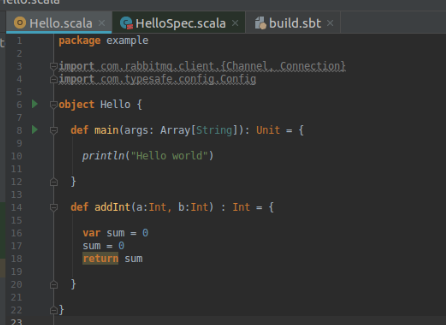
\includegraphics[width=3.42in,height=2.49in]{./media/image15.png}
	\end{Center}
\end{figure}


%%%%%%%%%%%%%%%%%%%% Figure/Image No: 14 Ends here %%%%%%%%%%%%%%%%%%%%

\par

Dans le chemin src/test/scala/example, on créé une classe « HelloSpec » :\par



%%%%%%%%%%%%%%%%%%%% Figure/Image No: 15 starts here %%%%%%%%%%%%%%%%%%%%

\begin{figure}[H]
	\begin{Center}
		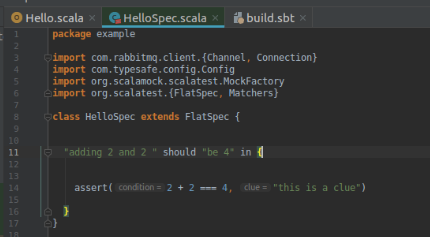
\includegraphics[width=3.83in,height=2.11in]{./media/image16.png}
	\end{Center}
\end{figure}


%%%%%%%%%%%%%%%%%%%% Figure/Image No: 15 Ends here %%%%%%%%%%%%%%%%%%%%

\par

Le plus important est de faire la configuration du fichier build.sbt :\par



%%%%%%%%%%%%%%%%%%%% Figure/Image No: 16 starts here %%%%%%%%%%%%%%%%%%%%

\begin{figure}[H]
	\begin{Center}
		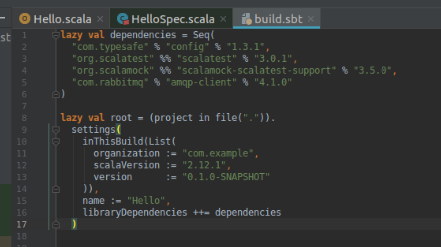
\includegraphics[width=3.88in,height=2.17in]{./media/image17.png}
	\end{Center}
\end{figure}


%%%%%%%%%%%%%%%%%%%% Figure/Image No: 16 Ends here %%%%%%%%%%%%%%%%%%%%

\par

On lance le sbt :\par



%%%%%%%%%%%%%%%%%%%% Figure/Image No: 17 starts here %%%%%%%%%%%%%%%%%%%%

\begin{figure}[H]
	\begin{Center}
		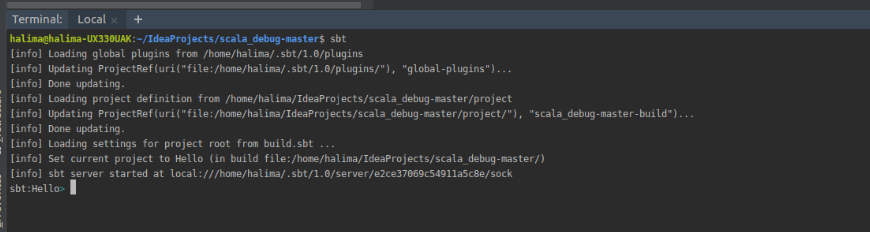
\includegraphics[width=5.63in,height=1.5in]{./media/image18.png}
	\end{Center}
\end{figure}


%%%%%%%%%%%%%%%%%%%% Figure/Image No: 17 Ends here %%%%%%%%%%%%%%%%%%%%

\par

Puis, on lance le scalaTest sur la classe de test :\par



%%%%%%%%%%%%%%%%%%%% Figure/Image No: 18 starts here %%%%%%%%%%%%%%%%%%%%

\begin{figure}[H]
	\begin{Center}
		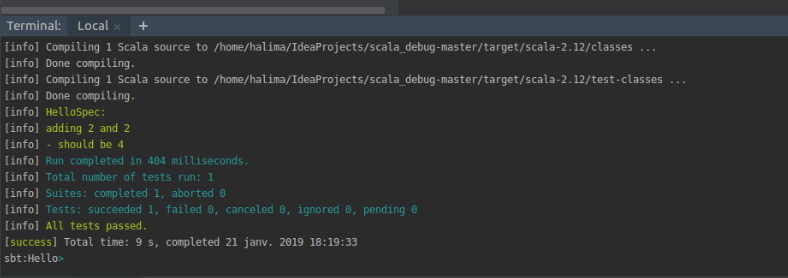
\includegraphics[width=5.54in,height=1.96in]{./media/image19.png}
	\end{Center}
\end{figure}


%%%%%%%%%%%%%%%%%%%% Figure/Image No: 18 Ends here %%%%%%%%%%%%%%%%%%%%

\par

Le test donne un résultat positif.\par

Si on change un chiffre au niveau du code, nous allons avoir un résultat de test négatif :\par



%%%%%%%%%%%%%%%%%%%% Figure/Image No: 19 starts here %%%%%%%%%%%%%%%%%%%%

\begin{figure}[H]
	\begin{Center}
		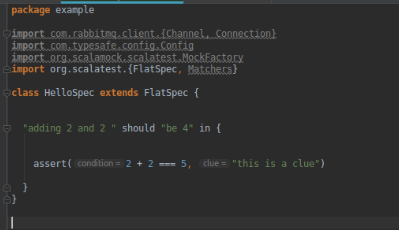
\includegraphics[width=4.16in,height=2.4in]{./media/image20.png}
	\end{Center}
\end{figure}


%%%%%%%%%%%%%%%%%%%% Figure/Image No: 19 Ends here %%%%%%%%%%%%%%%%%%%%

\par



%%%%%%%%%%%%%%%%%%%% Figure/Image No: 20 starts here %%%%%%%%%%%%%%%%%%%%

\begin{figure}[H]
	\begin{Center}
		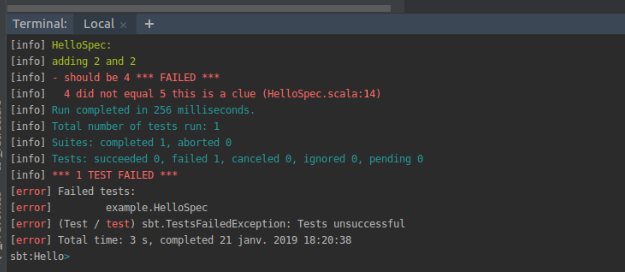
\includegraphics[width=5.37in,height=2.34in]{./media/image21.png}
	\end{Center}
\end{figure}


%%%%%%%%%%%%%%%%%%%% Figure/Image No: 20 Ends here %%%%%%%%%%%%%%%%%%%%

\par

\subsection{Sélection des styles de test pour votre projet}

\begin{justify}
ScalaTest prend en charge différents styles de test, chacun étant conçu pour répondre à un ensemble particulier de besoins. Pour vous aider à trouver les styles les mieux adaptés à votre projet, cette partie décrira les cas d'utilisation prévus pour chaque option.
\end{justify}\par

\begin{justify}
Nous allons utiliser un ensemble de styles de test pour chaque projet, Cela permet aux styles de test de s’adapter à l’équipe tout en maintenant l’uniformité dans la base de code du projet.
\end{justify}\par

\begin{justify}
Si vous préférez faire vos propres choix, nous vous donnerons un aperçu rapide des avantages et des inconvénients de chaque trait de style.
\end{justify}\par

\subsubsection{Style 1 : FunSuite}

\begin{justify}
{\fontsize{14pt}{16.8pt}\selectfont \textbf{\uline{Test01}}\par}
\end{justify}\par

\begin{justify}
Dans ce cas, la classe Test01 entend de org.scalatest.funsuite, dedans nous avons mis deux tests qui sont basics. 
\end{justify}\par



%%%%%%%%%%%%%%%%%%%% Figure/Image No: 21 starts here %%%%%%%%%%%%%%%%%%%%

\begin{figure}[H]
	\begin{Center}
		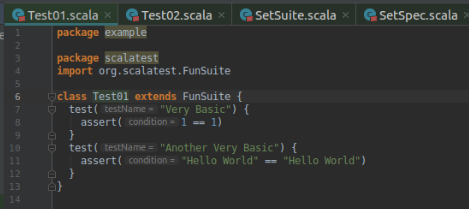
\includegraphics[width=4.89in,height=2.18in]{./media/image22.png}
	\end{Center}
\end{figure}


%%%%%%%%%%%%%%%%%%%% Figure/Image No: 21 Ends here %%%%%%%%%%%%%%%%%%%%

\par

\begin{justify}
‘test’ est une méthode défini dans Funsuite.
\end{justify}\par

\begin{justify}
Après exécution, les deux tests sont bien passés.
\end{justify}\par



%%%%%%%%%%%%%%%%%%%% Figure/Image No: 22 starts here %%%%%%%%%%%%%%%%%%%%

\begin{figure}[H]
	\begin{Center}
		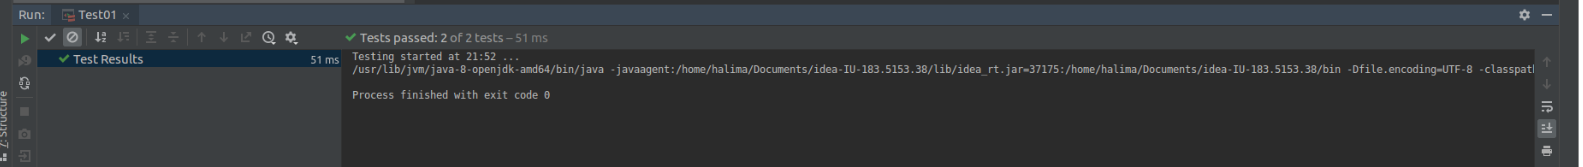
\includegraphics[width=6.3in,height=0.66in]{./media/image23.png}
	\end{Center}
\end{figure}


%%%%%%%%%%%%%%%%%%%% Figure/Image No: 22 Ends here %%%%%%%%%%%%%%%%%%%%

\par

\begin{justify}
{\fontsize{14pt}{16.8pt}\selectfont \textbf{\uline{Test02}}\par}
\end{justify}\par

\begin{justify}
Pareil pour la classe test02, mais maintenant nous avons introduit une erreur dans l’un des deux tests.
\end{justify}\par



%%%%%%%%%%%%%%%%%%%% Figure/Image No: 23 starts here %%%%%%%%%%%%%%%%%%%%

\begin{figure}[H]
	\begin{Center}
		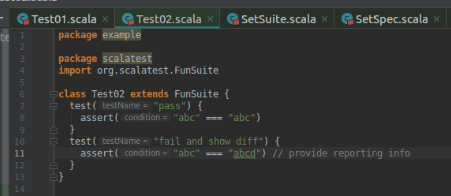
\includegraphics[width=4.7in,height=2.04in]{./media/image24.png}
	\end{Center}
\end{figure}


%%%%%%%%%%%%%%%%%%%% Figure/Image No: 23 Ends here %%%%%%%%%%%%%%%%%%%%

\par

\begin{justify}
Après exécution, le premier test a réussi et le deuxième test n’a pas passé.
\end{justify}\par



%%%%%%%%%%%%%%%%%%%% Figure/Image No: 24 starts here %%%%%%%%%%%%%%%%%%%%

\begin{figure}[H]
	\begin{Center}
		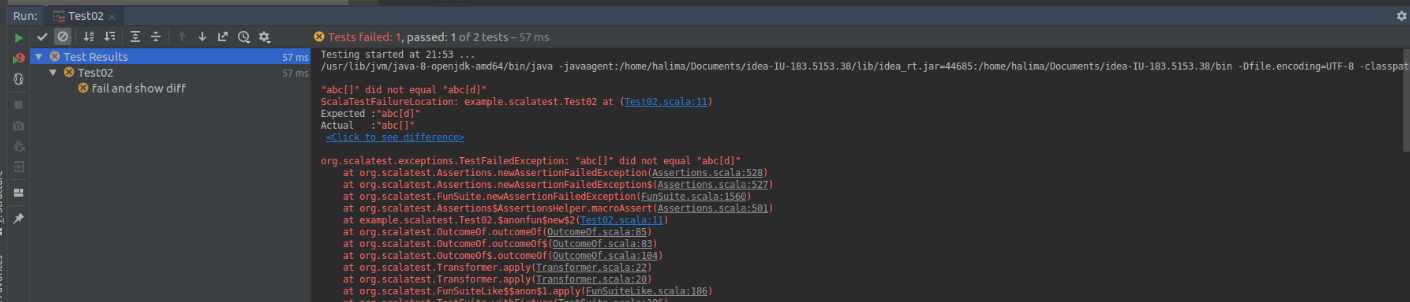
\includegraphics[width=6.3in,height=1.35in]{./media/image25.png}
	\end{Center}
\end{figure}


%%%%%%%%%%%%%%%%%%%% Figure/Image No: 24 Ends here %%%%%%%%%%%%%%%%%%%%

\par

\begin{justify}
Il existe d’autres styles qu’on peut appliquer sur les classes de test à part le FunSuite.
\end{justify}\par

\begin{justify}
Vers\ la suite je vais les citer, et je vais donner également un exemple d’application pour chacun.  
\end{justify}\par

\subsubsection{Style 2 : FlatSpec}

\begin{justify}
FlatSpec est une bonne première étape pour passer de xUnit à BDD. Sa structure est plate comme xUnit, très simple et familière, mais les noms de test doivent être écrits dans un style de spécification : "X should Y", "A must B", etc.
\end{justify}\par



%%%%%%%%%%%%%%%%%%%% Figure/Image No: 25 starts here %%%%%%%%%%%%%%%%%%%%

\begin{figure}[H]
	\begin{Center}
		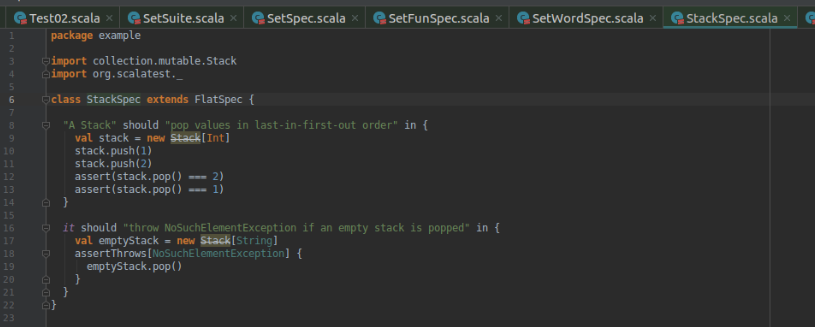
\includegraphics[width=6.3in,height=2.53in]{./media/image26.png}
	\end{Center}
\end{figure}


%%%%%%%%%%%%%%%%%%%% Figure/Image No: 25 Ends here %%%%%%%%%%%%%%%%%%%%

\par

\begin{justify}
Après exécution, les deux tests sont bien passés.
\end{justify}\par



%%%%%%%%%%%%%%%%%%%% Figure/Image No: 26 starts here %%%%%%%%%%%%%%%%%%%%

\begin{figure}[H]
	\begin{Center}
		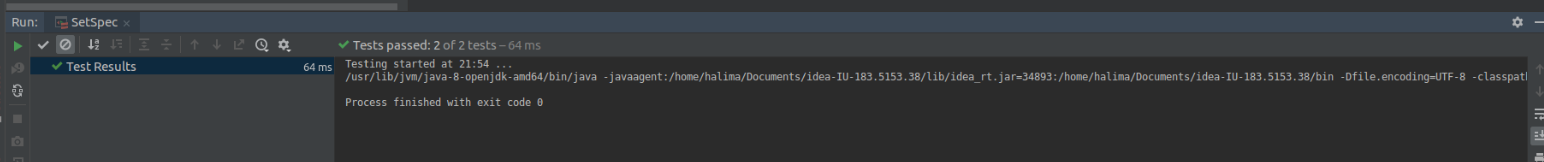
\includegraphics[width=6.3in,height=0.66in]{./media/image27.png}
	\end{Center}
\end{figure}


%%%%%%%%%%%%%%%%%%%% Figure/Image No: 26 Ends here %%%%%%%%%%%%%%%%%%%%

\par

\begin{justify}
Ensuite, on essaye de modifier le code pour le tester, du coup je remplace :
\end{justify}\par

\begin{justify}
 ‘ assert(stack.pop() === 1)’\  par ‘ assert(stack.pop() === 5)’ 
\end{justify}\par



%%%%%%%%%%%%%%%%%%%% Figure/Image No: 27 starts here %%%%%%%%%%%%%%%%%%%%

\begin{figure}[H]
	\begin{Center}
		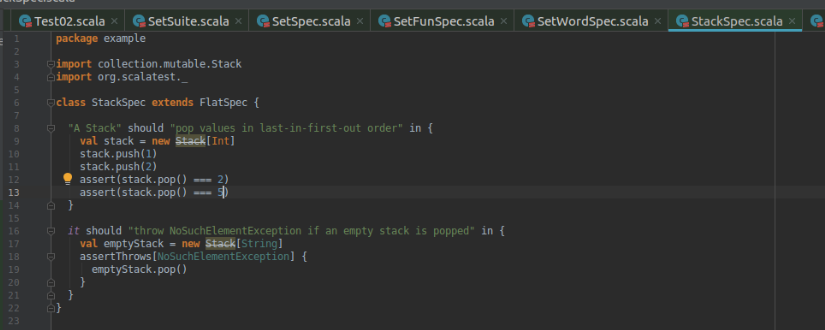
\includegraphics[width=6.3in,height=2.52in]{./media/image28.png}
	\end{Center}
\end{figure}


%%%%%%%%%%%%%%%%%%%% Figure/Image No: 27 Ends here %%%%%%%%%%%%%%%%%%%%

\par

\begin{justify}
Après exécution, un test est passé sur deux.
\end{justify}\par



%%%%%%%%%%%%%%%%%%%% Figure/Image No: 28 starts here %%%%%%%%%%%%%%%%%%%%

\begin{figure}[H]
	\begin{Center}
		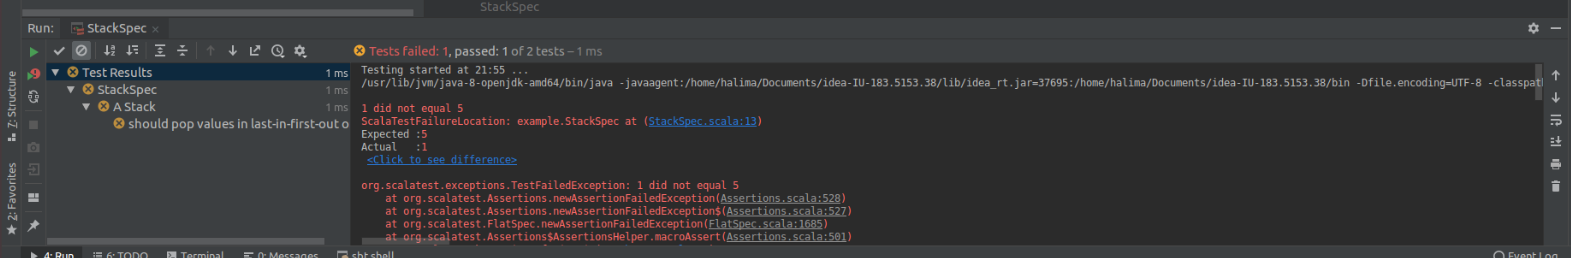
\includegraphics[width=6.3in,height=1.03in]{./media/image29.png}
	\end{Center}
\end{figure}


%%%%%%%%%%%%%%%%%%%% Figure/Image No: 28 Ends here %%%%%%%%%%%%%%%%%%%%

\par

\subsubsection{Style 3 : FunSpec}

\begin{justify}
Trait qui facilite un style de développement « basé sur le comportement », dans lequel les tests sont combinés avec du texte qui spécifie le comportement que les tests vérifient.
\end{justify}\par



%%%%%%%%%%%%%%%%%%%% Figure/Image No: 29 starts here %%%%%%%%%%%%%%%%%%%%

\begin{figure}[H]
	\begin{Center}
		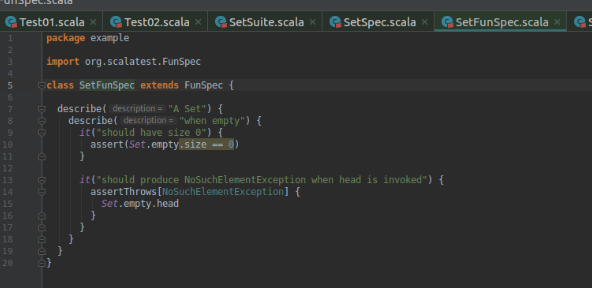
\includegraphics[width=5.06in,height=2.46in]{./media/image30.png}
	\end{Center}
\end{figure}


%%%%%%%%%%%%%%%%%%%% Figure/Image No: 29 Ends here %%%%%%%%%%%%%%%%%%%%

\par



%%%%%%%%%%%%%%%%%%%% Figure/Image No: 30 starts here %%%%%%%%%%%%%%%%%%%%

\begin{figure}[H]
	\begin{Center}
		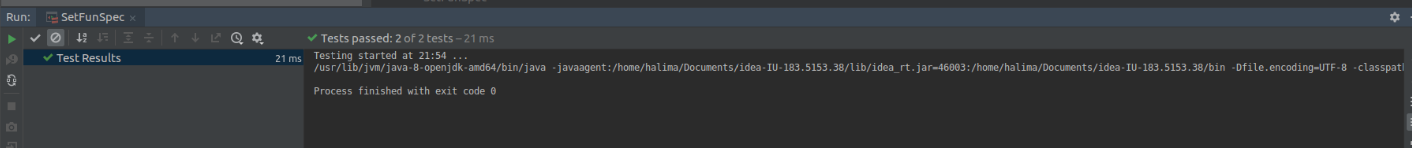
\includegraphics[width=6.3in,height=0.66in]{./media/image31.png}
	\end{Center}
\end{figure}


%%%%%%%%%%%%%%%%%%%% Figure/Image No: 30 Ends here %%%%%%%%%%%%%%%%%%%%

\par

\subsubsection{Style 4 : WordSpec}

\begin{justify}
WordSpec constitue souvent le moyen le plus naturel de transférer des tests specsN vers ScalaTest. WordSpec est très prescriptif dans la façon dont le texte doit être écrit. 
\end{justify}\par

Ce Trait WordSpec est ainsi nommé parce que votre texte de spécification est structuré en plaçant des mots après des chaînes.\par



%%%%%%%%%%%%%%%%%%%% Figure/Image No: 31 starts here %%%%%%%%%%%%%%%%%%%%

\begin{figure}[H]
	\begin{Center}
		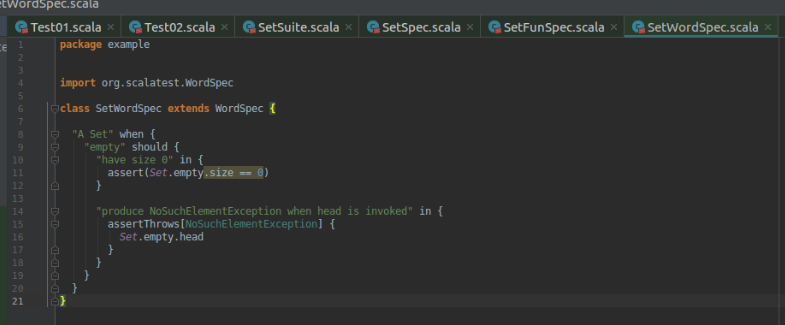
\includegraphics[width=6.3in,height=2.61in]{./media/image32.png}
	\end{Center}
\end{figure}


%%%%%%%%%%%%%%%%%%%% Figure/Image No: 31 Ends here %%%%%%%%%%%%%%%%%%%%

\par



%%%%%%%%%%%%%%%%%%%% Figure/Image No: 32 starts here %%%%%%%%%%%%%%%%%%%%

\begin{figure}[H]
	\begin{Center}
		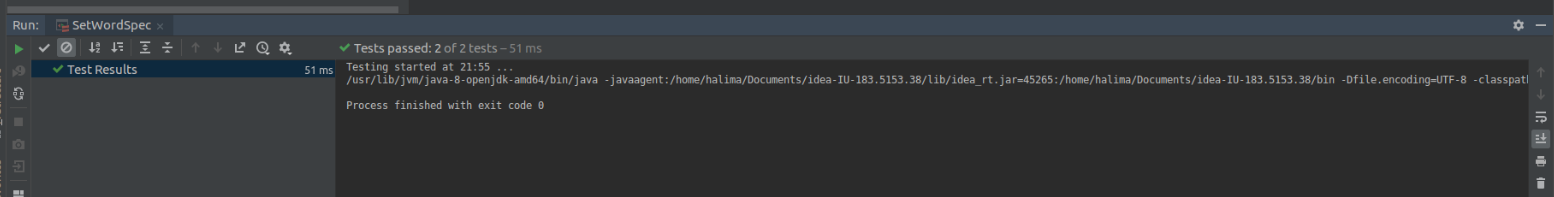
\includegraphics[width=6.3in,height=0.8in]{./media/image33.png}
	\end{Center}
\end{figure}


%%%%%%%%%%%%%%%%%%%% Figure/Image No: 32 Ends here %%%%%%%%%%%%%%%%%%%%

\par


\vspace{\baselineskip}
\subsubsection{Style 5 : FreeSpec}

\begin{justify}
Ce Trait facilite un style de développement « basé sur le comportement », dans lequel les tests sont imbriqués dans des clauses de texte dénotées avec l'opérateur de tiret (-).
\end{justify}\par



%%%%%%%%%%%%%%%%%%%% Figure/Image No: 33 starts here %%%%%%%%%%%%%%%%%%%%

\begin{figure}[H]
	\begin{Center}
		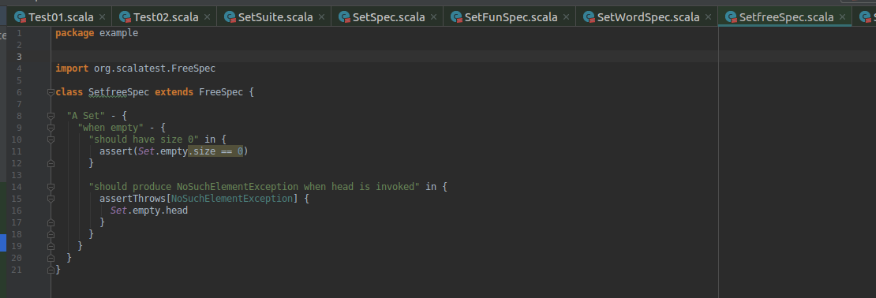
\includegraphics[width=6.3in,height=2.14in]{./media/image34.png}
	\end{Center}
\end{figure}


%%%%%%%%%%%%%%%%%%%% Figure/Image No: 33 Ends here %%%%%%%%%%%%%%%%%%%%

\par



%%%%%%%%%%%%%%%%%%%% Figure/Image No: 34 starts here %%%%%%%%%%%%%%%%%%%%

\begin{figure}[H]
	\begin{Center}
		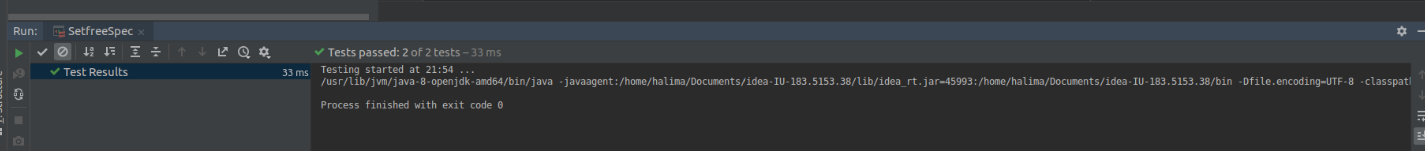
\includegraphics[width=6.3in,height=0.67in]{./media/image35.png}
	\end{Center}
\end{figure}


%%%%%%%%%%%%%%%%%%%% Figure/Image No: 34 Ends here %%%%%%%%%%%%%%%%%%%%

\par

\subsubsection{Style 6 : PropSpec}

\begin{justify}
Une suite de tests basés sur les propriétés.
\end{justify}\par

\begin{justify}
Ce trait facilite un style de test dans lequel chaque test est composé d'une vérification de propriété. Les tests sont enregistrés via une méthode "property", et reçoivent un nom et un corps.
\end{justify}\par



%%%%%%%%%%%%%%%%%%%% Figure/Image No: 35 starts here %%%%%%%%%%%%%%%%%%%%

\begin{figure}[H]
	\begin{Center}
		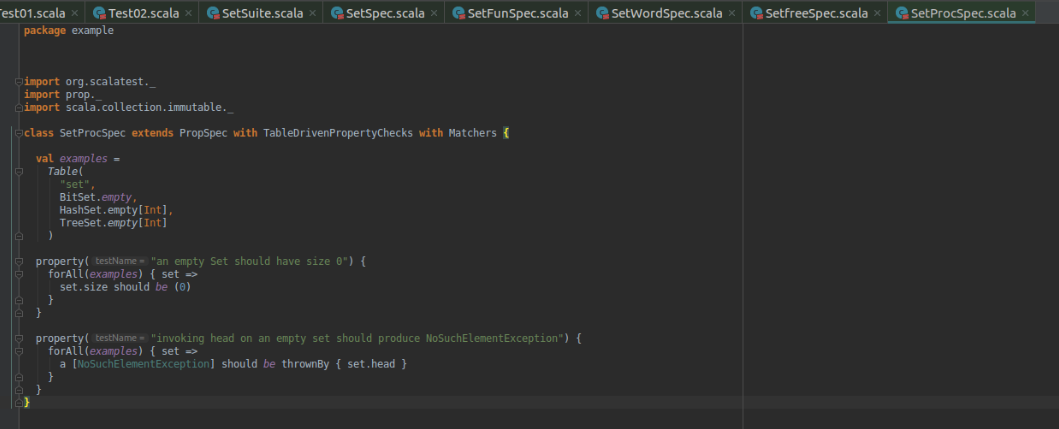
\includegraphics[width=6.3in,height=2.55in]{./media/image36.png}
	\end{Center}
\end{figure}


%%%%%%%%%%%%%%%%%%%% Figure/Image No: 35 Ends here %%%%%%%%%%%%%%%%%%%%

\par



%%%%%%%%%%%%%%%%%%%% Figure/Image No: 36 starts here %%%%%%%%%%%%%%%%%%%%

\begin{figure}[H]
	\begin{Center}
		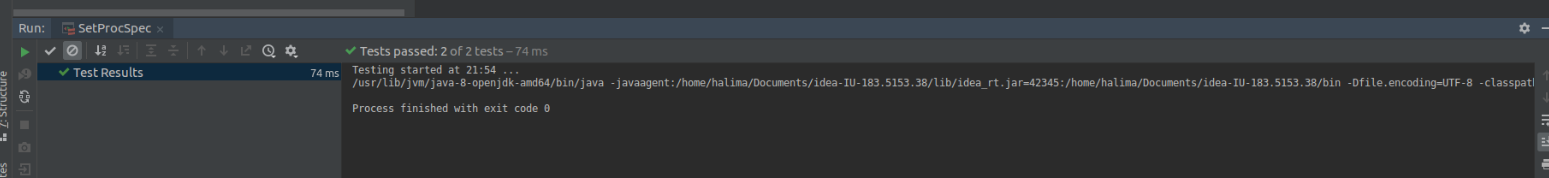
\includegraphics[width=6.3in,height=0.72in]{./media/image37.png}
	\end{Center}
\end{figure}


%%%%%%%%%%%%%%%%%%%% Figure/Image No: 36 Ends here %%%%%%%%%%%%%%%%%%%%

\par


\printbibliography
\end{document}